\documentclass{beamer}

\mode<presentation>
\usepackage{amsmath,amssymb,mathtools}
\usepackage{textcomp}
\usepackage{gensymb}
\usepackage{adjustbox}
\usepackage{subcaption}
\usepackage{enumitem}
\usepackage[utf8]{inputenc}
\usepackage{amssymb}
\usepackage{newunicodechar}
\usepackage{enumitem}
\setlist{nosep} % optional: removes vertical gaps
\setlist[enumerate]{label=\arabic*)} % custom numbering if you want

\newunicodechar{√}{$\sqrt{\;}$}
\newunicodechar{✅}{\checkmark}
\newunicodechar{❌}{\texttimes}
\usepackage{multicol}
\usepackage{listings}
\usepackage{url}
\usepackage{graphicx} % <-- needed for images
\def\UrlBreaks{\do\/\do-}

\usetheme{Boadilla}
\usecolortheme{lily}
\setbeamertemplate{footline}{
  \leavevmode%
  \hbox{%
  \begin{beamercolorbox}[wd=\paperwidth,ht=2ex,dp=1ex,right]{author in head/foot}%
    \insertframenumber{} / \inserttotalframenumber\hspace*{2ex}
  \end{beamercolorbox}}%
  \vskip0pt%
}
\setbeamertemplate{navigation symbols}{}

\lstset{
  frame=single,
  breaklines=true,
  columns=fullflexible,
  basicstyle=\ttfamily\tiny   % tiny font so code fits
}

\numberwithin{equation}{section}

% ---- your macros ----
\providecommand{\nCr}[2]{\,^{#1}{#2}}
\providecommand{\nPr}[2]{\,^{#1}P_{#2}}
\providecommand{\mbf}{\mathbf}
\providecommand{\pr}[1]{\ensuremath{\Pr\left(#1\right)}}
\providecommand{\qfunc}[1]{\ensuremath{Q\left(#1\right)}}
\providecommand{\sbrak}[1]{\ensuremath{{}\left[#1\right]}}
\providecommand{\lsbrak}[1]{\ensuremath{{}\left[#1\right.}}
\providecommand{\rsbrak}[1]{\ensuremath{\left.#1\right]}}
\providecommand{\brak}[1]{\ensuremath{\left(#1\right)}}
\providecommand{\lbrak}[1]{\ensuremath{\left(#1\right.}}
\providecommand{\rbrak}[1]{\ensuremath{\left.#1\right)}}
\providecommand{\cbrak}[1]{\ensuremath{\left\{#1\right\}}}
\providecommand{\lcbrak}[1]{\ensuremath{\left\{#1\right.}}
\providecommand{\rcbrak}[1]{\ensuremath{\left.#1\right\}}}
\theoremstyle{remark}
\newtheorem{rem}{Remark}
\newcommand{\sgn}{\mathop{\mathrm{sgn}}}
\providecommand{\abs}[1]{\left\vert#1\right\vert}
\providecommand{\res}[1]{\Res\displaylimits_{#1}}
\providecommand{\norm}[1]{\lVert#1\rVert}
\providecommand{\mtx}[1]{\mathbf{#1}}
\providecommand{\mean}[1]{E\left[ #1 \right]}
\providecommand{\fourier}{\overset{\mathcal{F}}{ \rightleftharpoons}}
\providecommand{\system}{\overset{\mathcal{H}}{ \longleftrightarrow}}
\providecommand{\dec}[2]{\ensuremath{\overset{#1}{\underset{#2}{\gtrless}}}}
\newcommand{\myvec}[1]{\ensuremath{\begin{pmatrix}#1\end{pmatrix}}}
\let\vec\mathbf
% ---------------------

\title{Matgeo Presentation - Problem 5.8.19}
\author{ee25btech11021 - Dhanush sagar}

\begin{document}
	

		




%---------------- Title Page ----------------
\begin{frame}
  \titlepage
\end{frame}

%---------------- Problem Statement ----------------
\begin{frame}{Problem Statement}
Let $a, b, c$ be real numbers. Consider the following system of equations in $x, y, z$:
\begin{align*}
\frac{x^2}{a^2} + \frac{y^2}{b^2} - \frac{z^2}{c^2} &= 1, \\
\frac{x^2}{a^2} - \frac{y^2}{b^2} + \frac{z^2}{c^2} &= 1, \\
-\frac{x^2}{a^2} + \frac{y^2}{b^2} + \frac{z^2}{c^2} &= 1.
\end{align*}
The system has:
\begin{enumerate}
    \item no solution
    \item unique solution
    \item infinitely many solutions
    \item finitely many solutions
\end{enumerate}
\end{frame}

%---------------- Mathematical Formula ----------------
\begin{frame}{solution}

Let
\begin{align}
A &= \frac{x^2}{a^2}, \\
B &= \frac{y^2}{b^2}, \\
C &= \frac{z^2}{c^2}.
\end{align}

Then the system becomes
\begin{align}
A + B - C &= 1, \\
A - B + C &= 1, \\
- A + B + C &= 1.
\end{align}
\end{frame}
\begin{frame}{solution}
The augmented matrix is
\begin{align}
\myvec{1 & 1 & -1 & 1 \\ 1 & -1 & 1 & 1 \\ -1 & 1 & 1 & 1}
&\xrightarrow{R_2 \to R_2 - R_1}
\myvec{1 & 1 & -1 & 1 \\ 0 & -2 & 2 & 0 \\ -1 & 1 & 1 & 1}
\xrightarrow{R_3 \to R_3 + R_1}
\myvec{1 & 1 & -1 & 1 \\ 0 & -2 & 2 & 0 \\ 0 & 2 & 0 & 2} \notag\\
&\xrightarrow{R_3 \to R_3 + R_2}
\myvec{1 & 1 & -1 & 1 \\ 0 & -2 & 2 & 0 \\ 0 & 0 & 2 & 2} 
\xrightarrow{R_2 \to -\frac{1}{2} R_2} 
\myvec{1 & 1 & -1 & 1 \\ 0 & 1 & -1 & 0 \\ 0 & 0 & 2 & 2} \notag\\
&\xrightarrow{R_3 \to \frac{1}{2} R_3} 
\myvec{1 & 1 & -1 & 1 \\ 0 & 1 & -1 & 0 \\ 0 & 0 & 1 & 1} 
\xrightarrow{R_2 \to R_2 + R_3} 
\myvec{1 & 1 & -1 & 1 \\ 0 & 1 & 0 & 1 \\ 0 & 0 & 1 & 1} \notag\\
&\xrightarrow{R_1 \to R_1 + R_3} 
\myvec{1 & 1 & 0 & 2 \\ 0 & 1 & 0 & 1 \\ 0 & 0 & 1 & 1} 
\xrightarrow{R_1 \to R_1 - R_2} 
\myvec{1 & 0 & 0 & 1 \\ 0 & 1 & 0 & 1 \\ 0 & 0 & 1 & 1}.
\end{align}
\end{frame}
\begin{frame}{solution}
From the final matrix we read
\begin{align}
A &= 1, & B &= 1, & C &= 1.
\end{align}

Therefore,
\begin{align}
\frac{x^2}{a^2} &= 1, & \frac{y^2}{b^2} &= 1, & \frac{z^2}{c^2} &= 1,
\end{align}
which gives
\begin{align}
x &= \pm a, & y &= \pm b, & z &= \pm c.
\end{align}

Hence there are $2^3=8$ distinct solutions for $(x,y,z)$, so the correct choice is
\begin{align}
\boxed{\text{(d) finitely many solutions}}
\end{align}

\end{frame}
%---------------- C Source Code ----------------
\begin{frame}[fragile]{C Source Code:fraction matrix.c}
\begin{verbatim}
#include <stdio.h>

void gen_system_points(double *A, double *B) {
    // Coefficient matrix (3x3)
    double tempA[9] = {
         1,  1, -1,   // Eqn 1
         1, -1,  1,   // Eqn 2
        -1,  1,  1    // Eqn 3
    };
    // RHS vector
    double tempB[3] = {1, 1, 1};

    for (int i = 0; i < 9; i++) A[i] = tempA[i];
    for (int i = 0; i < 3; i++) B[i] = tempB[i];
}




\end{verbatim}
\end{frame}

%---------------- Python solve.py ----------------
\begin{frame}[fragile]{Python Script:fraction matrix.py}
\begin{verbatim}
import ctypes
import numpy as np
import itertools
# --- Load C shared library ---
lib = ctypes.CDLL("./gen_system_points.so")
lib.gen_system_points.argtypes = [ctypes.POINTER(ctypes.c_double), ctypes.POINTER(ctypes.c_double)]
# Storage
A_storage = (ctypes.c_double * 9)()
B_storage = (ctypes.c_double * 3)()
lib.gen_system_points(A_storage, B_storage)
# Convert to numpy
A = np.array(A_storage).reshape(3, 3)
B = np.array(B_storage)
print("Coefficient matrix A:\n", A)
print("RHS vector B:\n", B)
# Solve AX = B
X, Y, Z = np.linalg.solve(A, B)

\end{verbatim}
\end{frame}

\begin{frame}[fragile]{Python Script:fraction matrix.py}
\begin{verbatim}
print("\nSolution (X,Y,Z) = ({}, {}, {})".format(X, Y, Z))
# Symbolic answer
symbolic_points = []
for sx, sy, sz in itertools.product([1, -1], repeat=3):
    symbolic_points.append((f"{'+' if sx>0 else '-'}a",
                            f"{'+' if sy>0 else '-'}b",
                            f"{'+' if sz>0 else '-'}c"))
print("\nSymbolic solutions (in terms of a,b,c):")
for p in symbolic_points:
    print(p)
a, b, c = 2.0, 3.0, 1.0   # change these values
numeric_points = [(sx*a, sy*b, sz*c) for sx, sy, sz in itertools.product([1,-1],[1,-1],[1,-1])]
print("\nNumeric solutions (for a={}, b={}, c={}):".format(a, b, c))
for p in numeric_points:
    print(p)
np.savetxt("points_abc.txt", numeric_points)
print("\nSaved numeric points to points_abc.txt")
\end{verbatim}
\end{frame}


\begin{frame}[fragile]{Python Script: plot matrix.py}
\begin{verbatim}
import numpy as np
import matplotlib.pyplot as plt
# Parameters
a = b = c = 1.0  # main intersection point
# Meshgrid for planes
xx = np.linspace(0, 1.5, 30)
yy = np.linspace(0, 1.5, 30)
XX, YY = np.meshgrid(xx, yy)
# Plane equations
Z1 = XX + YY - 1       # X + Y - Z = 1
Z2 = 1 - XX + YY       # X - Y + Z = 1
Z3 = 1 + XX - YY       # -X + Y + Z = 1
# Plot
fig = plt.figure(figsize=(10,8))
ax = fig.add_subplot(111, projection='3d')
# Plot planes with low opacity
ax.plot_surface(XX, YY, Z1, color="red", alpha=0.2)



\end{verbatim}
\end{frame}
\begin{frame}[fragile]{Python Script: plot matrix.py}
\begin{verbatim}
ax.plot_surface(XX, YY, Z2, color="green", alpha=0.2)
ax.plot_surface(XX, YY, Z3, color="blue", alpha=0.2)
# Add plane equations as text
ax.text(1.3, 0.2, Z1[0,-1], "X + Y - Z = 1", color='red', fontsize=12)
ax.text(1.3, 0.2, Z2[0,-1], "X - Y + Z = 1", color='green', fontsize=12)
ax.text(1.3, 0.2, Z3[0,-1], "-X + Y + Z = 1", color='blue', fontsize=12)
# Plot the single intersection point (1,1,1)
ax.scatter(1,1,1, color='red', s=200, edgecolor='black', label='Point (1,1,1)')
# Annotate the intersection point
ax.text(1.02, 1.02, 1.02, "(1,1,1)", fontsize=12, color='red')
# Axes labels
ax.set_xlabel("X = x²/a²")
ax.set_ylabel("Y = y²/b²")
ax.set_zlabel("Z = z²/c²")
ax.set_title("Planes with Single Intersection Point Highlighted")
ax.legend()
plt.show()

\end{verbatim}
\end{frame}

\begin{frame}{Result Plot}
 \begin{figure}[H]
     \centering
     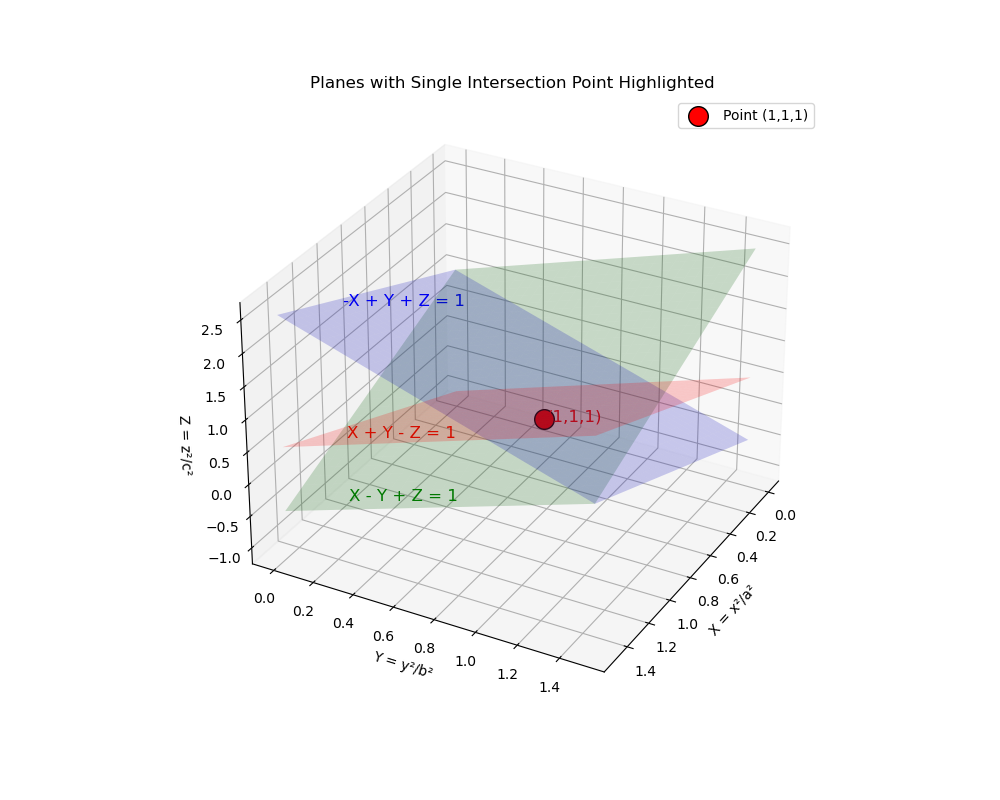
\includegraphics[width=0.8\columnwidth]{figs/fig1.png}
     \caption*{}
     \label{fig:fig1}
 \end{figure}
 
\end{frame}
\end{document}

